\section{Consultar Auxiliar}

Un paciente podrá consultar los auxiliares que tiene asociados a
su cuenta permitiéndole saber los datos personales del auxiliar y saber los tratamientos del cual se hará cargo.

\subsubsection{Procedimiento}
\begin{enumerate}
	
	\item Da clic en el icono \textbf{Auxiliares} de la pantalla \textbf{Menú Principal}.

		\begin{figure}[!htbp]			\hypertarget{fig:mpPaciente7}{\hspace{1pt}}
		\begin{center}
			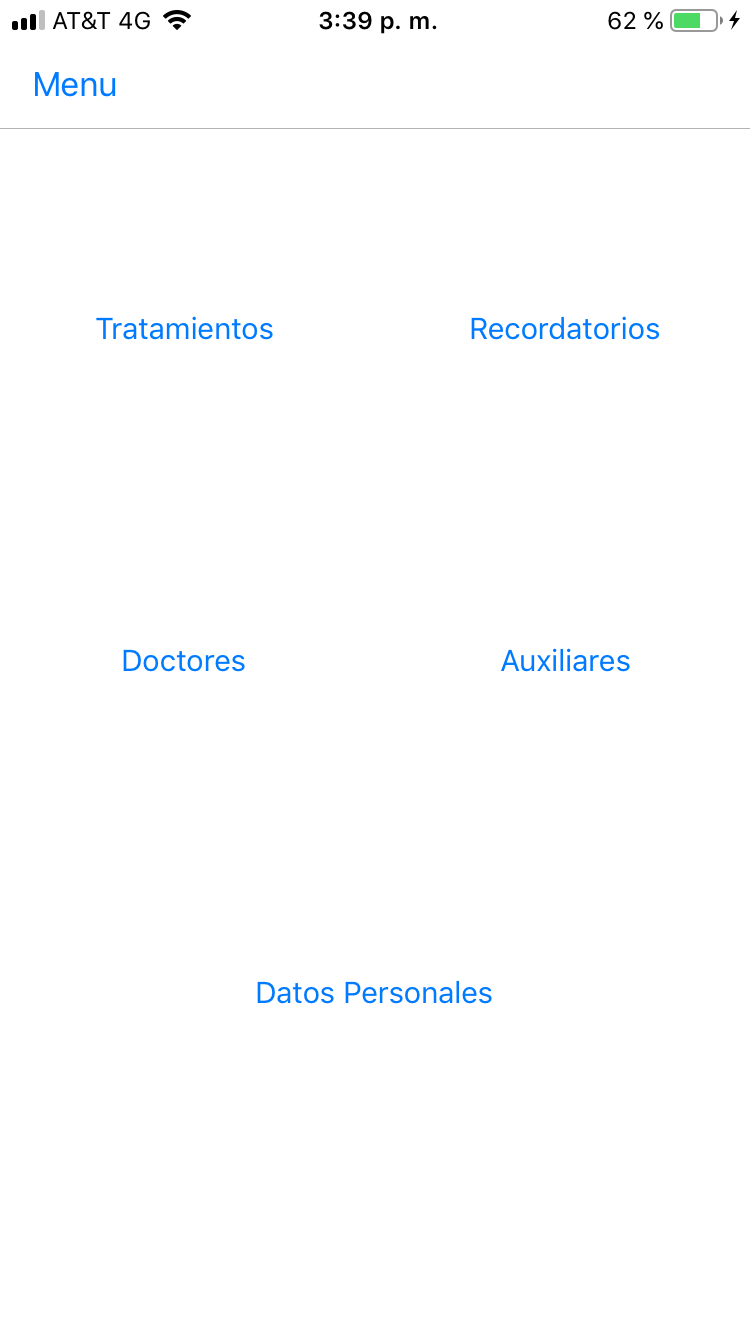
\includegraphics[height=0.4\textheight]{Paciente/ConsultarAuxiliar/images/mpPaciente}
			\caption{Menú Principal Paciente}
			\label{fig:mpPaciente7}
		\end{center}
	\end{figure}

	\item Se mostrará la pantalla \textbf{Auxiliares}. 
	\newpage
	\begin{figure}[!htbp]			
		\hypertarget{fig:Auxiliares2}{\hspace{1pt}}
		\begin{center}
			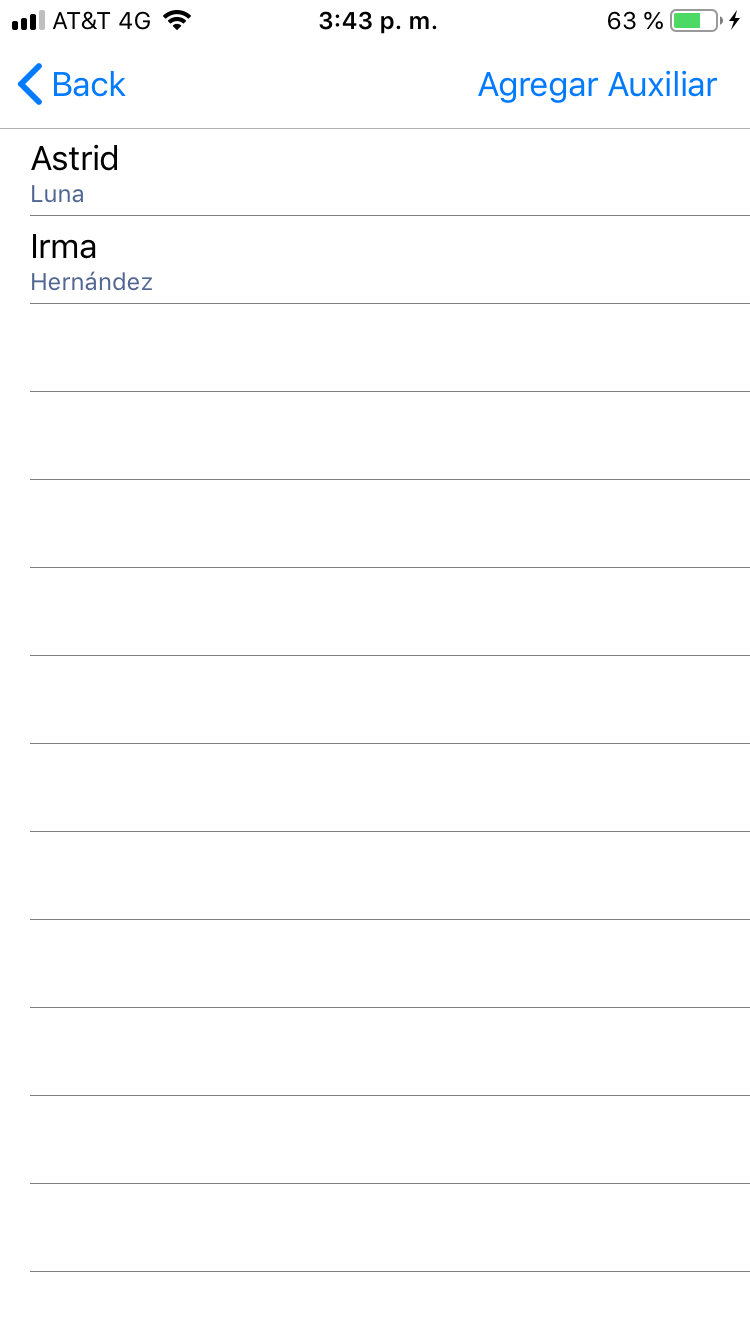
\includegraphics[height=0.4\textheight]{Paciente/ConsultarAuxiliar/images/Auxiliares}
			\caption{Auxiliares}
			\label{fig:Auxiliares2}
		\end{center}
	\end{figure}

\end{enumerate}

